\documentclass[10pt]{standalone}
\usepackage{commands}

\begin{document}
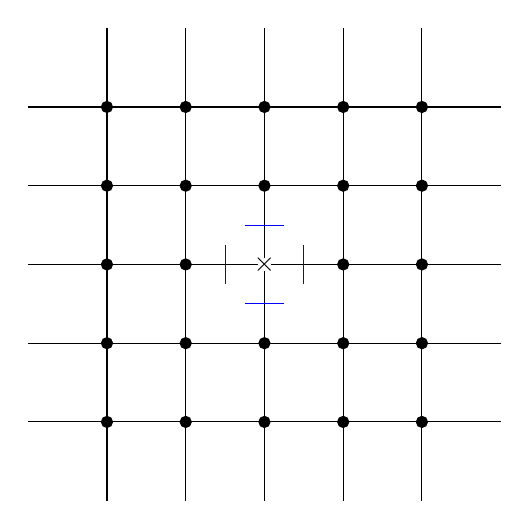
\begin{tikzpicture}
    \foreach \j in {1,...,5} {
            \draw[] (-1, \j) -- (5, \j);
    };
    \foreach \i in {0,...,4} {
        \foreach \j in {1,...,5} {
            \filldraw (\i, \j) circle (2pt);
        }
        \draw[] (\i, 0) -- (\i, 6);
    };
    \filldraw[draw=white, fill=white] (2, 3) circle (2.1pt);
    \node[] at (2, 3) {$\times$};
    \draw[blue] (1.75, 3.5) -- (2.25, 3.5);
    \draw[blue] (1.75, 2.5) -- (2.25, 2.5);
    \draw[blue] (1.5, 2.75) -- (1.5, 3.25);
    \draw[blue] (2.5, 2.75) -- (2.5, 3.25);
\end{tikzpicture}
\end{document}